\documentclass[12pt, oneside]{book}
\title{A Guide to the Spanish Subjunctive}
\author{Krithika Ravishankar}

\usepackage{float}
\usepackage[margin=1in]{geometry}
\usepackage{tgpagella}
\usepackage[T1]{fontenc}


\makeatletter
\def\l@table{\@dottedtocline{1}{1.5em}{3em}}
\makeatother\usepackage{amssymb}

\usepackage{tocbibind}
\usepackage{enumitem}
\usepackage{xcolor}
\usepackage{booktabs}
\usepackage[colorlinks=false]{hyperref}
\hypersetup{
	linkbordercolor = {cyan},
}
\usepackage{appendix}

\usepackage[normalem]{ulem}
\setlength\parindent{0pt}
\newcommand{\nye}{\~{n}}
\newcommand{\exc}{\textexclamdown}
\newcommand{\arr}{$\rightarrow$}
\newcommand{\ita}[1]{\textit{#1}}
\newenvironment{conf}[1]
    {\begin{center}
		\begin{tabular}{|p{0.9\textwidth}|}
		\hline\\
		\large\textbf{#1} \\
	}
    { 
	    \\\\\hline
	    \end{tabular} 
	    \end{center}
    }

\usepackage{xparse}
\ExplSyntaxOn

\NewDocumentCommand{\conjugation}{O{}m}
 {
  \group_begin:
  \keys_set:nn { froggos/conjugation } { #1 }
  \froggos_conjugation:n { #2 }
  \group_end:
 }

\keys_define:nn { froggos/conjugation }
 {
  placement    .tl_set:N  = \l__froggos_conjugation_placement_tl,
  placement    .initial:n = H,
  caption      .tl_set:N  = \l__froggos_conjugation_caption_tl,
  shortcaption .tl_set:N  = \l__froggos_conjugation_shortcaption_tl,
  label        .tl_set:N  = \l__froggos_conjugation_label_tl,
 }

\seq_new:N \l__froggos_conjugation_entries_seq

\cs_new_protected:Nn \froggos_conjugation:n
 {
  \tl_if_empty:NF \l__froggos_conjugation_caption_tl
   {
    \__froggos_conjugation_table_begin:V \l__froggos_conjugation_placement_tl
    \centering
   }
  \seq_set_split:Nnn \l__froggos_conjugation_entries_seq { \\ } { #1 }
  \begin{tabular}{ll}
    \toprule
    \textbf{Form} & \textbf{Conjugation} \\
    \midrule
    \textit{Yo}       & \textit{\seq_item:Nn \l__froggos_conjugation_entries_seq {1}} \\
    \textit{T\'u}     & \textit{\seq_item:Nn \l__froggos_conjugation_entries_seq {2}} \\
    \textit{\'El/Ella/Ud.}     & \textit{\seq_item:Nn \l__froggos_conjugation_entries_seq {3}} \\
    \textit{Nosotr@s} & \textit{\seq_item:Nn \l__froggos_conjugation_entries_seq {4}} \\
    \textit{Vosotr@s} & \textit{\seq_item:Nn \l__froggos_conjugation_entries_seq {5}} \\
    \textit{Ell@s/Uds.}    & \textit{\seq_item:Nn \l__froggos_conjugation_entries_seq {6}} \\
    \bottomrule
  \end{tabular}
  \tl_if_empty:NF \l__froggos_conjugation_caption_tl
   {
    \tl_if_empty:NTF \l__froggos_conjugation_shortcaption_tl
     {
      \caption{\l__froggos_conjugation_caption_tl}
     }
     {
      \caption[\l__froggos_conjugation_shortcaption_tl]{\l__froggos_conjugation_caption_tl}
     }
    \tl_if_empty:NF \l__froggos_conjugation_label_tl
     {
      \label{\l__froggos_conjugation_label_tl}
     }
    \end{table}
   }
 }

\cs_new_protected:Nn \__froggos_conjugation_table_begin:n
 {
	 \begin{table}[#1]
 }
\cs_generate_variant:Nn \__froggos_conjugation_table_begin:n {V}

\ExplSyntaxOff


\usepackage{tikz}
\pagestyle{headings}


\definecolor{gre}{rgb}{0,0.5,0.3}
\definecolor{eye}{rgb}{0.29,0.33,0.13}

\usetikzlibrary{calc,trees,positioning,arrows,fit,shapes,calc}

\begin{document}
\sloppy
\maketitle
\tableofcontents
\listoftables
\chapter{Welcome!}

Hello, eager student!\\

For most readers, the subjunctive \textit{mood} (not \textit{tense}, we'll get into that) is one of the most challenging aspects of the Spanish language. \\

This guide is designed for a native English speaker learning Spanish. Why read it? This is the condensed version of everything you'll need to know to use and understand the subjunctive mood confidently. This guide tries to clear up some common misconceptions around the spooky subjunctive and is meant for an advanced student. \\

It assumes you already know how to work with the indicative mood (which you probably already know if you're reading this). This guide covers the vast majority of what you'll need to know regarding the subjunctive.  \\

Let's dive in!

\vfill
{\footnotesize Copyright \textcopyright\ 2019 Krithika Ravishankar}


\chapter{Introduction}
What is the subjunctive? \\

It's a mood, so it reflects the speaker's ... mood. In Spanish, there are three different moods: the indicative, the subjunctive, and the imperative.
\begin{conf}{Mood versus Tense}
 A super common mistake is to call the subjunctive a tense, but a tense is only used to refer to time. Yes, you'll hear instructors sometimes refer to a ``subjunctive tense,'' in which case they're probably referring to something called the present subjunctive. Yes, they're wrong, but it's just a technicality. 
\end{conf}
The indicative mood probably comprises most of what you've seen so far. It's used for when the speaker is pretty certain about what they're talking about. For instance, if I were to say ``It's going to rain tomorrow,'' that would imply that I'm pretty sure it's going to rain. Hence, we'd translate that as \textit{Va a llover ma{\nye}ana} or \textit{Llover\'{a} ma{\nye}ana}. \\

The imperative mood is used to tell someone to do something, like a command or an order. For example, to tell your friend to ``hurry up,'' we would use the imperative mood. That sentence would translate to \textit{{\exc}Ap\'{u}rate ya!}, \textit{{\exc}Ten prisa!}, or \textit{{\exc}Date prisa!}. \\

Now, let's talk about the subjunctive mood. The subjunctive mood is the \underline{exact} opposite of the indicative mood. While the indicative mood was used to express certainty, the subjunctive mood is used to express uncertainty. For instance, to say that you wished you had studied harder, you would need to use the subjunctive. The sentence \textit{I wish I had studied harder} can be translated as \textit{Ojal\'{a} que hubiera estudiado m\'{a}s}. Notice that we didn't use the indicative and say \textit{hab\'{i}a estudiado}. \\

We'll talk more about when to use the subjunctive in the next chapters, but mostly in the \hyperref[sec:weirdo]{WEIRDO Clauses} section and in the \hyperref[sec:other]{Other Phrases} sections.\\

There's a list of tenses and moods in the \hyperref[subsec:tense]{List of Tenses and Moods} section in the Appendix. If the stuff that we've gone over so far is 100\% new to you, I recommend taking a look at that list before we move on. \\

Let's talk about how to conjugate in the subjunctive in the next chapter. 






\chapter{Conjugation}
In this chapter, we're just going to talk about how to conjugate verbs in the subjunctive mood. We're not going to discuss when to use which forms; that's covered in later sections. For now, we shall conjugate like machines. \\

\section{Present Subjunctive}
To conjugate \textit{most} verbs in the present subjunctive, we can follow the following steps:
\begin{enumerate}[noitemsep]
	\item Find the \textit{yo} form of the verb in the present indicative
	\item Remove the \ita{-o} ending (this is the ``stem'')
	\item Add the appropriate swapped ending in the present indicative
\end{enumerate}

What is this ``swapped ending?'' Remember how we have \textit{-ar}, \textit{-er}, and \textit{-ir} verbs? We're going to split those three categories into two categories, where all \textit{-ar} verbs make up their own category, and all \textit{-er} and \textit{-ir} verbs are clubbed into one category. When we use a ``swapped ending,'' it means that:
\begin{itemize}[noitemsep]
	\item If we have an \textit{-ar} verb, we conjugate it like an \textit{-er} verb in the present indicative
	\item If we have an \textit{-er} or an \textit{-ir} verb, we conjugate it like an \textit{-ar} verb in the present indicative
	\item If we're conjugating in the \textit{yo} form, just use the third-person singular form (the \textit{{\'{e}l, ella, usted}} form)
\end{itemize}

If that didn't make much sense, that's okay. Let's do a few examples, and then you might want to revisit the two previous paragraphs. They'll make a lot more sense after these examples: \\

Let's conjugate the verb \textit{tener} (to have) in the \textit{nosotr@s} form of the present subjunctive:
\begin{enumerate}[noitemsep]
	\item The \ita{yo} form of \ita{tener} is \ita{tengo}
	\item Let's remove the \ita{o}. We're left with \ita{teng-}
	\item Now we just need to add the right swappend ending. Since \ita{tener} is an \ita{-er} verb, we need to use the \ita{-ar} ending, which is \ita{-amos} in the \ita{nosotr@s} form. Now we have \ita{tengamos}, which is our final result. 
\end{enumerate}

Let's conjugate the verb \ita{caer} (to fall) in the \ita{yo} form of the present subjunctive:
\begin{enumerate}[noitemsep]
	\item The \ita{yo} form of \ita{caer} is \ita{caigo}
	\item Let's remove the \ita{o}. We're left with \ita{caig-}
	\item Now we just need to add the right swappend ending. Since \ita{caer} is an \ita{-er} verb, we need to use the \ita{-ar} ending, which is \ita{-a} in the \ita{yo} form. Why is it \ita{-a} instead of \ita{-o}? It's because we're conjugating in the \ita{yo} form. You might want to take a look at bullet \#3 earlier in the chapter for clarification. Now we have \ita{caiga}, which is our final result. 
\end{enumerate}

Let's conjugate the verb \ita{atravesar} (to cross) in the \ita{ellos} form of the present subjunctive:
\begin{enumerate}[noitemsep]
	\item The \ita{yo} form of \ita{atravesar} is \ita{atravieso}
	\item Let's remove the \ita{o}. We're left with \ita{atravies-}
	\item Now we just need to add the right swappend ending. Since \ita{atravesar} is an \ita{-ar} verb, we need to use the \ita{-er} ending, which is \ita{-en} in the \ita{ellos} form. Now we have \ita{atraviesen}, which is our final result. 
\end{enumerate}

\begin{conf}{Stem Changes}
	For stem-changing verbs (in the present tense), we do \underline{not} change the stem in the \ita{nosotr@s} or \ita{vosotr@s} forms. 
\end{conf}

Hence, the full conjugation of \ita{atravesar} in the present subjunctive is as follows: 
\conjugation[
  caption=Present subjunctive conjugation of \textit{atravesar},
  label=verb:atravesar,
]{atraviese \\ atravieses  \\ atraviese  \\ atravesemos \\ atraves\'eis  \\ atraviesen}

\begin{conf}{Spelling Changes}
Something to keep in mind would be any spelling changes. In the preterit, remember how we had to change the spelling for \ita{-car}, \ita{-gar}, \ita{-zar}, and \ita{-guar} verbs? Well, those same changes apply in the present subjunctive. It's not as complicated as it seems, if you can remember that the Spanish language loves to keep its pronunciation regular, and will change the spelling of certain words to make sure the language is phonetic. It's actually a blessing, if you think about it. If you're curious about the reasons why there are spelling changes, there's a section about it in the \hyperref[subsec:pronun]{Pronunciation and Spelling Rules} part of the appendix. 
\end{conf}

Spelling change example:
Let's conjugate the verb \ita{pegar} (to hit or to glue) in the \ita{t{\'{u}}} form of the present subjunctive:
\begin{enumerate}[noitemsep]
	\item The \ita{yo} form of \ita{pegar} is \ita{pego}
	\item Let's remove the \ita{o}. We're left with \ita{peg-}
	\item Now we just need to add the right swappend ending. Since \ita{pegar} is an \ita{-ar} verb, we need to use the \ita{-er} ending, which is \ita{-es} in the \ita{t{\'{u}}} form. Now we have \sout{\ita{peges}}. Hey, wait a sec! That's not right! Since it's a \ita{-gar} verb, we need to add a \ita{u} after the \ita{g}. Now we have \ita{pegues}, which is our final result.
\end{enumerate}

We're not done yet, though. What we just covered is how we conjugate \ita{most} verbs. There are still some that march to their own beat: \\



\begin{table}[ht]
\centering
\begin{tabular}[t]{ll}
\toprule
\textbf{Verb} & \textbf{Stem} \\
\midrule
	\ita{saber} & \ita{sepa}\\
	\ita{estar} & \ita{est{\'{e}}}\\
	\ita{dar} & \ita{d{\'e}}\\
	\ita{haber} & \ita{haya}\\
	\ita{ser} & \ita{sea} \\
	\ita{ir} & \ita{vaya} \\
	\bottomrule
%\label{List of irregular verbs in the Present Subjunctive}

\end{tabular}
	\caption{{\label{tab:irrpres}}List of irregular verbs in the present subjunctive}
\end{table}

After getting the stem, you'll just need to tag on the ending. 
\begin{conf}{Accent Marks}
	For \ita{estar} (to be) and \ita{dar} (to give), you'll need to adjust the accent marks following the accent mark rules, which you can read up in the \hyperref[subsec:pronun]{Pronunciation and Spelling Rules} part of the appendix. If you don't want to read that, that's okay. I've left the conjugations anyway if you prefer to just memorize the conjugations for these two verbs.
\end{conf}

\conjugation[
  caption=Present subjunctive conjugation of \textit{estar},
  label=verb:estar,
]{est\'e \\ est\'es  \\ est\'e  \\ estemos \\ est\'eis \\ est\'en}

\conjugation[
	caption=Present subjunctive conjugation of \textit{dar},
  label=verb:dar,
]{d\'e \\ des  \\ d\'e  \\ demos \\ deis \\ den}




For reference, the "at" sign (@, or the \ita{arroba}) is informally used to make terms gender neutral; don't use this for anything formal, like written work. That's why in the previous conjugation charts I used \ita{ell@s} in the place of \ita{ellos} and \ita{ellas}. 
%%%%%%%%%%%%%%%%%%%%%%%%%%%%%%%%%%%%%%%%%%%%%%%%%%%%%%%%%%%%%%%%%%%%%%%%%%%%%


\section{Subjunctive Imperfect}

The next thing that we're going to go over are the conjugations in the subjunctive imperfect. A cool thing about this verb tense is that there are \ita{zero} exceptions to the rules given below, which is pretty rare. \\

There are two sets of conjugations in the subjunctive imperfect, the \ita{-ra} (called the type 1 endings) or the \ita{-se} (called the type 2 endings). Within this section, I'm going to refer to them as the \ita{-ra} endings or the \ita{-se} endings for consistency. We pretty much exclusively use the \ita{-ra} forms in conversation, while in writing, both the \ita{-ra} and the \ita{-se} forms are used.\\

\subsection{Type 1 (\ita{-ra}) Endings}
Let's first talk about how we conjugate with \ita{-ra} endings: 
\begin{enumerate}[noitemsep]
	\item Find the \ita{ell@s, Uds.} form of the verb in the preterit
	\item Remove the \ita{-ron} ending (leaving you with the ``stem'')
	\item Add the appropriate ending given below. 
\end{enumerate}
\

\conjugation[
	caption=Type 1/(\ita{-ra}) endings in the subjunctive imperfect
]{-ra \\ -ras \\ -ra \\ \normalfont{Accent +} -ramos \\ -rais \\ -ran}


What does ``Accent + \ita{-amos}'' mean in the \ita{nosotr@s} form? Remember to add an accent mark to the last syllable of the stem before adding the ending. Why do we need to add an accent? It's to make sure that syllable remains stressed. A more in-depth explanation is given in the \hyperref[subsec:pronun]{Pronunciation and Spelling Rules} part of the appendix. \\

Let's conjugate a sample verb, \ita{poder} (to be able):
\begin{enumerate}[noitemsep]
	\item The \ita{ell@s, Uds.} form of \ita{poder} is \ita{pudieron}
	\item Let's remove the \ita{ron}. We're left with \ita{pudie-}
	\item The final step is to add the endings (see below). Pay attention to the \ita{nosotr@s} form. 
\end{enumerate}


\conjugation[
	caption=Conjugations of \ita{poder} in the subjunctive imperfect (\ita{-ra})
]{pudiera \\ pudieras \\ pudiera \\ pudi\'eramos \\ pudierais \\ pudieran}

Let's conjugate another verb, \ita{hablar} (to talk/speak) for funsies: 

\begin{enumerate}[noitemsep]
	\item The \ita{ell@s, Uds.} form of \ita{hablar} is \ita{hablaron}
	\item Let's remove the \ita{ron}. We're left with \ita{habla-}
	\item The final step is to add the endings (see below). Pay attention to the \ita{nosotr@s} form. 
\end{enumerate}

\conjugation[
	caption=Conjugations of \ita{hablar} in the subjunctive imperfect (\ita{-ra})
]{hablara \\ hablaras \\ hablara \\ habl\'aramos \\ hablarais \\ hablaran}

\subsection{Type 2 (\ita{-se}) Endings}

Now let's talk about how we conjugate with \ita{-se} endings. The process is fairly similar to conjugating with \ita{-ra} endings. The only thing that differs are the endings we add to the stem. \\

\begin{enumerate}[noitemsep]
	\item Find the \ita{ell@s, Uds.} form of the verb in the preterit
	\item Remove the \ita{-ron} ending (leaving you with the ``stem'')
	\item Add the appropriate ending given below. 
\end{enumerate}

\conjugation[
	caption=Type 2/(\ita{-se}) endings in the subjunctive imperfect
]{-se \\ -ses \\ -se \\ \normalfont{Accent +} -semos \\ -seis \\ -sen}


We're going to conjugate the same two verbs (\ita{poder} and \ita{hablar}), but this time with the \ita{-se} endings. \\

Let's conjugate a sample verb, \ita{poder} (to be able):
\begin{enumerate}[noitemsep]
	\item The \ita{ell@s, Uds.} form of \ita{poder} is \ita{pudieron}
	\item Let's remove the \ita{ron}. We're left with \ita{pudie-}
	\item The final step is to add the endings (see below). Pay attention to the \ita{nosotr@s} form. 
\end{enumerate}

\conjugation[
	caption=Conjugations of \ita{poder} in the subjunctive imperfect (\ita{-se})
]{pudiese \\ pudieses \\ pudiese \\ pudi\'esemos \\ pudieseis \\ pudiesen}



Let's conjugate another verb, \ita{hablar} (to talk/speak) for funsies: 

\begin{enumerate}[noitemsep]
	\item The \ita{ell@s, Uds.} form of \ita{hablar} is \ita{hablaron}
	\item Let's remove the \ita{ron}. We're left with \ita{habla-}
	\item The final step is to add the endings (see below). Pay attention to the \ita{nosotr@s} form. 
\end{enumerate}

\conjugation[
	caption=Conjugations of \ita{hablar} in the subjunctive imperfect (\ita{-se})
]{hablase \\ hablases \\ hablase \\ habl\'asemos \\ hablaseis \\ hablasen}
%%%%%%%%%%%%%%%%%%%%%%%%%%%%%%%%%%%%%%%%%%%%%%%%%%%%%%%%%%%%%%%%%%%%%%%%%%%%%%%%%%%%%%%%%%%%%%%%%%%%%%%%%%%%%%%%%%%%%%%%
\section{The Perfect Tenses}

The subjunctive perfect tenses work in the same way that perfect tenses worked in the indicative. All conjugations take the form of \ita{haber} + past participle.\\ 

Here are the conjugations of the verb \ita{haber} in the subjunctive: 


	\begin{table}[H]
	\centering
	\begin{tabular}{lllll}
		\toprule
		& \textbf{Present} & \textbf{Imperfect: \ita{-ra}} &\textbf{ Imperfect: \ita{-se}} & \textbf{Future} \\
		\midrule
		\ita{\textbf{Yo}}  & \ita{haya} & \ita{hubiera} & \ita{hubiese} & \ita{hubiere} \\
		\ita{\textbf{T{\'u}}} & \ita{hayas} & \ita{hubieras} & \ita{hubieses} & \ita{hubieres}\\
		\ita{\textbf{{\'E}l, Ella, Ud.}} & \ita{haya} & \ita{hubiera} & \ita{hubiese} & \ita{hubiere}\\
		\ita{\textbf{Nosotr@s}} & \ita{hayamos} & \ita{hubi{\'e}ramos} & \ita{hubi{\'e}semos} & \ita{hubi{\'e}remos} \\
		\ita{\textbf{Vosotr@s}} & \ita{hay{\'a}is} & \ita{hubierais} & \ita{hubieseis} & \ita{hubiereis} \\
		\ita{\textbf{Ell@s, Uds.}} & \ita{hayan} & \ita{hubieran} & \ita{hubiesen} & \ita{hubieren}\\
		\bottomrule
	\end{tabular}
		\caption{{\label{tab:perfect}}Conjugations of \ita{haber} in the subjunctive}
\end{table}
%%%%%%%%%%%%%%%%%%%%%%%%%%%%%%%%%%%%%%%%%%%%%%%%%%%%%%%%%%%%%%%%%%%%%%%%%%%%%%%%%%%%%%%%%%%%%%%%%%%%%%%%%%%%%%%%%%%5%%%%
\section{The Subjunctive Future (Optional)}

This verb tense is used pretty rarely. You'll see it used exclusively in legal documents and other extremely formal pieces of literature, so it's okay if you skip this section and move on to the next chapter. However, if you're curious, read on! \\

This verb tense also won't be discussed for the rest of the guide, so I'm also going to talk about its usage as well as conjugation in this section. The subjunctive future is (sparingly) used to indicate uncertainty in the future, and is typically replaced by the present subjunctive in the vast majority of cases. \\

Conjugations are similar to what we saw in the subjunctive imperfect: 
\begin{enumerate}[noitemsep]
	\item Find the \ita{ell@s, Uds.} form of the verb in the preterit
	\item Remove the \ita{-ron} ending (leaving you with the ``stem'')
	\item Add the appropriate ending given below. 
\end{enumerate}

\conjugation[
	caption=Endings in the subjunctive future
]{-re \\ -res \\ -re \\ \normalfont{Accent +} -remos \\ -reis \\ -ren}

Let's conjugate an example verb, \ita{leer} (to read):
\begin{enumerate}[noitemsep]
	\item The \ita{ell@s, Uds.} form of \ita{leer} is \ita{leyeron}
	\item Let's remove the \ita{ron}. We're left with \ita{leye-}
	\item The final step is to add the endings (see below). Pay attention to the \ita{nosotr@s} form. 
\end{enumerate}

\conjugation[
	caption=Conjugations of \ita{leer} in the subjunctive future
]{leyere \\ leyeres \\ leyere \\ ley\'eremos \\ leyereis \\ leyeren}




\chapter{Conjugation Practice}
Conjugate the following verbs in the present subjunctive in all forms. Answers are given in the \hyperref[sec:ans]{Answers} section.

\begin{itemize}[before=\itshape,font=\normalfont,noitemsep]
	\item Tener
	\item Dar
	\item Saber
	\item Averiguar
	\item Poner
	\item Escribir
	\item Levantar
	\item Bajar
	\item Hacer
	\item Colocar
	\item Empezar
	\item Leer
\end{itemize}

Conjugate the following verbs in the subjunctive imperfect, in both the \ita{-ra} and the \ita{-se} forms:
\begin{itemize}[before=\itshape,font=\normalfont,noitemsep]
	\item Entender
	\item Ser
	\item Andar
	\item Estar
	\item Convertir
	\item Decir
	\item Venir
	\item Saber
	\item Bailar
	\item Querer
\end{itemize}


\chapter{WEIRDO Clauses}
\label{sec:weirdo}
In this chapter, we're going to talk about when to use the subjunctive mood. 


\begin{conf}{The Big Idea}
If you get nothing else from this guide, please at least walk away with this: the subjunctive mood is used to express uncertainty. Sometimes rules will require you to use the subjunctive, and sometimes the use of the subjunctive is left to the speaker's discretion. Regardless of how and/or why it is used, the subjunctive will add an element of uncertainty or doubt to the sentence. 
\end{conf}

 WEIRDO is a common acronym that's used to teach students when to use the subjunctive mood instead of the indicative. \\ 

As an overview, this is what WEIRDO stands for:
\begin{itemize}[noitemsep]
	\item W: Wishes
	\item E: Emotional Expressions
	\item I: Impersonal Expressions
	\item R: Recommendations
	\item D: Doubt \& Denial
	\item O: \ita{Ojal{\'a}}
\end{itemize}

There are typically two clauses in a sentence uses the subjunctive, a main clause that's in the indicative, and a subordinate clause that's in the subjunctive. If the main clause happens to be a WEIRDO clause, then there's really high chance that you'll need to use the subjunctive in the subordinate clause. In this section, we'll pretty much exclusively be dealing with cases where the main clause is a WEIRDO clause. \\

The tense of the main clause determines the tense of the subordinate clause: 
\begin{itemize}[noitemsep]
	\item If the main clause is in the present tense, the subordinate clause can be in the present subjunctive or in the present imperfect; it depends on when the event is supposed to happen
		\begin{itemize}[noitemsep]
			\item If the event is supposed to happen in the present or future, use the present subjunctive
			\item If the event was supposed to happen in the past, use the subjunctive imperfect
		\end{itemize}
	\item If the main clause is in the preterit/imperfect, the subordinate clause in the subjunctive imperfect
	\item If the main clause is in the conditional, the subordinate clause is in the subjunctive imperfect
	\item Following the above three statements: if the WEIRDO clause is in a perfect tense, choose the appropriate subjunctive perfect tense
\end{itemize}

Finally, these are the most common features of sentences that use the subjunctive:
\begin{itemize}[noitemsep]
	\item A relative pronoun, typically \ita{que} (what), but could also include \ita{quien} (who), \ita{donde} (where), or \ita{cuando} (when) \footnote{Don't confuse these with interrogative pronouns, like \ita{qu{\'e}} (what), \ita{qui{\'e}n} (who), \ita{d{\'o}nde} (where), or \ita{cu{\'a}ndo} (when), which are used to form questions. Relative pronouns are used to provide additional information. For instance, in the sentence, ``I'm looking for someone who speaks Arabic well,'' the word ``who'' is a relative pronouns that provides extra information about the individual. In Spanish, that same sentence would be translated as \ita{Busco a alguien que hable bien el {\'a}rabe}, taking the subjunctive. }
	\item There are two subjects (one for each clause)
	\item One WEIRDO clause, and a subordinate clause
\end{itemize}

For the rest of the guide, when I say that an expression``triggers'' the subjunctive, I mean that the expression requires the subjunctive to be used. \\

Don't worry if this stuff doesn't make that much sense right now. It'll make more sense after we've gone through a few examples in the subsequent sections. \\

Let's dive in! 

\begin{conf}{Get caffeinated!}
Seriously. If you're kinda tired right now, take a nap before reading this. If you're wide awake, you might want to pour yourself a cup of coffee, tea, or Diet Coke before reading the next few sections. This is the part that can and hopefully will mentally fatigue you. If you go through the next few sections without at least getting kinda confused, there are two possibilities: (a) you already know all of this, or (b) you understood none of this. 
\end{conf}
\section{W: Wishes}

One use of the subjunctive is to express wishes. For example, to translate the sentence ``I hope you're doing okay,'' we would need to use the subjunctive, in saying \ita{Espero que est{\'e}s bien}. Let's break it down, point by point:

\begin{enumerate}
	\item Let's rewrite the sentence in an equivalent form: ``I hope that you're doing okay.'' In English, relative pronouns are sometimes optional, while in Spanish they're always required when linking clauses. Adding in the optional relative pronoun helps us see the two clauses.
	\item The first clause, the ``I hope'' part, is the WEIRDO clause, since it expresses a wish. Wishes are things that we're \underline{not sure} about, which expresses uncertainty. Since wishes are uncertain, this tells us that we'll need to use the subjunctive at some point in this translation, but not just yet. Since the speaker is sure that they're not sure (that's a mind-boggle, but stick with me here), that part of the sentence takes the indicative. That's the reason why we say \ita{Espero que} in the first part of the translated sentence. 
	\item After the relative pronoun \ita{que}, we get the subordinate clause. The speaker isn't really sure if the person they're addressing is actually okay, which is why we need to use the subjunctive here. Now, we have \ita{est{\'e}s bien}.
	\item Piecing that together, we now have \ita{Espero que est{\'e}s bien.}
\end{enumerate}

Woo-hoo! One down, with 50 gazillion more to go! Don't worry. You'll be able to do all that reasoning in a split-second with more practice. \\

Let's do another example with wishes. This time, we're translating the sentence ``They hoped she would pass the test.'' The translation for that would be \ita{Esperaban que aprobabara el examen. }\\

\begin{enumerate}
	\item Since we can't really see the relative pronoun in our sentence, let's rewrite it: ``They hoped that she would pass the test.''
	\item The first clause, the ``They hoped,'' is the WEIRDO clause, since it expresses a wish. Since the speakers don't know whether she passed the test, they have to use the subjunctive. With the subjunctive, a key thing to remember is to put yourself in the speaker's/speakers' shoes, and see how \underline{they} would feel, certain or uncertain about the outcome. 
	\item Again, like in the previous example, the speakers are sure that they're not sure. That's why the WEIRDO clause is always in the indicative. Hence, so far, we have \ita{Esperaban que} as the first part of the translation.
	\item After the relative pronoun \ita{que}, we get the subordinate clause. The speakers aren't really sure if she's passed the exam, which is why the use of the subjunctive is necessary. Remember the bit in the beginning of this subsection that talked about how the tense of the WEIRDO clause determines the tense of the subordinate clause? That becomes important in this case. Since the WEIRDO clause is in the imperfect, the verb in the subordinate clause has to be conjugated in the subjunctive imperfect. Now we have \ita{aprobara el examen} as the latter half of the translation.
	\item Piecing both together, we have \ita{Esperaban que aprobara el examen.}
\end{enumerate}

But wait! What if the first half of the sentence is in the present, but we want the latter half to be in the past tense? Just use the perfect tense. For example, to translate the sentence ``I hope you had a good summer,'' we'd say \ita{Espero que hayas pasado un buen verano}. \\

Finally, let's work through an example that does \underline{not} use the subjunctive. Let's translate the sentence ``He hopes to get into med school.'' \\

Why shouldn't we use the subjunctive? Let's go through our checklist (the set of bullets towards the beginning of the chapter):
\begin{itemize}[noitemsep]
	\item Is there a relative pronoun? Sure, if we rewrite our sentence as ``He hopes that he'll get into med school.''
	\item Are there two subjects? \underline{No!} In many (not all) cases, not having two different subjects is a pretty good reason to not use the subjunctive.
\end{itemize}

Here's what \underline{incorrect} \footnote{In linguistics, the only things that are wrong are things that native speakers would never say. I rant about this in the \hyperref[subsec:accents]{Accent Rules} section in the appendix.} reasoning would have looked like: 
\begin{enumerate}
	\item Rewriting the sentence with the relative pronoun, we'd get ``He hopes that he'll get into med school.''
	\item Translating the WEIRDO clause, we'd have \ita{\'El espera que} as the first chunk.
	\item After the relative pronoun, we'll need to translate the subordinate clause. Now, we'd get \ita{entre a la escuela de medicina} as the latter half.
	\item Piecing those together, we'll get the incorrect translation \ita{\'El espera que entre a la escuela de medicina.}
\end{enumerate}

So what's wrong with that? While it may be ``grammatically correct,'' (whatever that means) it's wrong for pretty much all intents and purposes, since native speakers wouldn't be inclined to say that sentence we just produced. \\

When we don't have two unique subjects, native speakers prefer to use the infinitive instead. Hence, the correct translation would really be \ita{\'El espera entrar a la escuela de medicina} (lit. He hopes to get into med school.)\\

\subsection{Wishes with \ita{que}}

This is not the most common usage of the subjunctive, but you'll still see it occasionally. The best way to understand this usage might be to look at a few examples sentences:

\begin{enumerate}[noitemsep]
	\item ``May they find happiness.'' \arr \ita{Que encuentren felicidad.} 
\end{enumerate}

We'll look into several more examples like these ones in the following sections, and you'll get a better feel for when to or when \underline{not} to use the subjunctive.
\section{E: Emotional Expressions}
%%%%%%%%%%%%%%%%%%%%%%%%%%%%%%%%%%%%%%%%%%%%%%%%%%%%%%%%%%%%%%%%%%%%%%%%%%%%%%%%%%%%%%%%%%%%%%%%%%%%%%
Emotional expressions with the subjunctive can be pretty challenging, just like expressions with doubt and denial. Emotional expressions express an opinion on an event, and are therefore subjective. That's why these expressions can trigger the subjunctive. \\

Let's look at some sample examples: 
\begin{enumerate}[noitemsep]
	\item ``I'm glad you came'' $\rightarrow$ \ita{Me alegro de que vinieras.} or \ita{Me alegro de que hayas venido.} \footnote{Another way of saying this could be with \ita{alegrar} instead of \ita{alegrarse de}.  Hence, additional translations would include \ita{Me alegra que hayas venido} and \ita{Me alegra que vinieras}.}
	\item ``They hate it when the park is crowded. '' or ``They hate it that the park is crowded.'' $\rightarrow$ \ita{Odian que el parque est\'e lleno} or \ita{Odian que el parque est\'a lleno}
	\item ``She's scared you'll fail the exam.'' $\rightarrow$ \ita{Teme que repruebes el examen.}
	\item ``I was so angry that he was ignoring us.'' $\ita{Estaba tan enfadada que nos ignorara.}$
	\item ``I'm so sorry that you were sick.'' $\rightarrow$ \ita{Lamento que estuvieras enfermo.}
\end{enumerate}

\begin{conf}{Rules? I don't know her.}
	This is the first (of five billion) instances where there are multiple right answers to a translation, where one translation uses the subjunctive, and the other uses the indicative. \underline{These statements are not synonymous.} While both are correct, they have different meanings. \\
	
\\	In some of these cases, we're required to use the subjunctive, and in others, we're required to use the indicative. In other cases, there aren't really any rules to guide us; the mood used depends on how factual/uncertain the speaker is about a statement. It's pretty important to realize which of the three scenarios apply to any given sentence, and the best way to get used to these kinds of things is to increase your exposure to the language. \\

\\ For this particular section, you'll need to use the subjunctive more often than not. For emotional expressions, the default usage is with the subjunctive, and if the speaker feels more certain, the mood can be changed from its default to the indicative. 
\end{conf}

Let's look at the first sentence, ``I'm glad you came.'' This one is pretty self-explanatory. 
\begin{enumerate}
	\item The first bit of the sentence becomes \ita{Me alegro de que}. 
	\item Since it's an emotional expression, we'll need to use the subjunctive in the subordinate clause, so the latter half of the sentence becomes \ita{vinieras} or \ita{hayas venido}. Here, we have a choice between the subjunctive imperfect and the present perfect, and you can pick whichever one you want. 
	\item Thus, the complete translation is \ita{Me alegro de que hayas venido} or \ita{Me alegro de que vinieras}.
\end{enumerate}

The second sentence gets a bit more fun, ``They hate it when the park is crowded.''
\begin{enumerate}
	\item First off, sentences like ``I like it when,'' ``We hate it when,'' ``It frustrates us when,'' all fall under emotional expressions in Spanish. Those three phrases can be translated as \ita{Me gusta que}, \ita{Odiamos que}, \ita{Nos frustra que}. Hence, the first bit of the translation becomes \ita{Odian que}.
	\item The second bit of the translation is also interesting. As we talked about earlier, this is one of those scenarios where you could technically use either mood. 
		\begin{itemize}
			\item If we use the subjunctive, it means that they just hate it when the park is crowded. It's a general statement, applying to whenever the park happens to be crowded. 
			\item If we use the indicative, it means that they hate it that the park is crowded, implying that the park is definitely crowded. This statement conveys more certainty, since it's said in reference to a definite event. 
		\end{itemize}
	\item Hence, we get two different translations, \ita{Odian que el parque est\'e lleno} or \ita{Odian que el parque est\'a lleno}. 
\end{enumerate}

The remaining example sentences follow the first example. Working them out is left as an exercise for the reader. 
\section{I: Impersonal Expressions}
%%%%%%%%%%%%%%%%%%%%%%%%%%%%%%%%%%%%%%%%%%%%%%%%%%%%%%%%%%%%%%%%%%%%%%%%%%%%%%%%%%%%%%%%%%%%%%%%%%%%%%%%%
This is one of the easiest uses of the subjunctive. \\

Impersonal expressions are statements that lack subjects. Here are a list of sample impersonal expressions along with their corresponding translations:
\begin{enumerate}[noitemsep]
	\item ``It's too hot today.'' $\rightarrow$ \ita{Hoy hace demasiado calor.}
	\item ``It's important to eat healthy and work out.'' $\rightarrow$ \ita{Es importante comer sano y hacer ejercicio}.
	\item ``It's important for you to eat healthy and work out.'' $\rightarrow$ \ita{Es importante que comas sano y que hagas ejercicio.}
	\item ``It's a pity that you were sick.'' $\rightarrow$ \ita{Es una l{\'a}stima que estuvieras enfermo.}
	\item ``It was the best of times, it was the worst of times ...'' $\rightarrow$ \ita{Era el mejor de los tiempos, era el peor de los tiempos ... } (Charles Dickens, \underline{A Tale of Two Cities})
\end{enumerate}

As you can see, some of those sentences used the subjunctive (the third and fourth statements), and the rest didn't. \\

How do we know if an impersonal expression will take the subjunctive or not? This bit is pretty simple. Are there two different subjects (one is null, the other is present)? If so, use the subjunctive. If not, just go with the infinitive. \\

One thing to keep in mind is that in English, we tend to use the preposition ``for,'' while in Spanish, in these sorts of situations, we use the relative pronoun \ita{que}. \\

With that in mind, let's take the third example in this section, the sentence ``It's important for you to eat healthy and work out.''
\begin{enumerate}
	\item In Spanish, the first bit of the translation is self-explanatory, we get \ita{Es importante}.
	\item Instead of the word ``for,'' we use \ita{que}. Since there's a definite subject associated with the second half of the sentence (you, or \ita{t\'u}), we conjugate the verbs in the present subjunctive.
	\item Hence, our final translation becomes \ita{Es importante que comas sano y que hagas ejercicio}. 
\end{enumerate}

Let's work through the fourth statement, ``It's a pity that you were sick.'' This follows similarly. 
\begin{enumerate}
	\item The first bit is translated as normal; ``It's a pity'' becomes \ita{Es una l\'astima}. Instead of the word ``for,'' we use \ita{que}. 
	\item Since there's a definite subject associated with the second half of the sentence (you, or \ita{t\'u}), we conjugate the verb. However, unlike the previous example, we need to conjugate our verb in the subjunctive imperfect. This is because the event of being sick occurred in the past (given the context of our sentence, we can assume that the person being addressed was sick in the past and is now okay).
	\item Hence, our final sentence becomes \ita{Es una l\'astima que estuvieras enfermo.}
\end{enumerate}

%%%%%%%%%%%%%%%%%%%%%%%%%%%%%%%%%%%%%%%%%%%%%%%%%%%%%%%%%%%%%%%%%%%%%%%%%%%%%%%%%%%%%%%%%%%5%%%%%%%%%%
\section{R: Recommendations}

The most common use of the subjunctive is in recommendations or suggestions. \\

If we want to tell someone to do something, we don't really have a guarantee that they'll actually do it. That's why the subjunctive is \underline{always} used in sentences with recommendations or suggestions, since we're not that sure about the outcome.\\

Let's start out by just listing some sample sentences with recommendations along with their corresponding translations:
\begin{enumerate}[noitemsep]
	\item ``My parents want me to plan more.'' $\rightarrow$ \ita{Mis padres quieren que planee m\'as.}
	\item ``I'd like for you to clean your room.'' $\rightarrow$ \ita{Me gustar\'ia que limpiaras tu cuarto.}
	\item ``The doctor advises you to avoid caffeine.'' $\rightarrow$ \ita{El doctor te aconseja que evites la cafe\'ina.}
	\item ``I already told you to start your homework!'' $\rightarrow$ \ita{\textexclamdown Ya te dije que empezaras tu tarea!}
	\item Like 50\% of the lyrics in Shakira's (feat. Alejandro Sanz) \ita{La Tortura}. \footnote{I highly recommend you to listen to this song to drill in the uses of the subjunctive with recommendations. Music in general is pretty good for drilling in concepts. }
\end{enumerate}

One thing to take note of is that in English, we tend to use the preposition ``to'' in these sorts of constructions. For example, we can say ``The doctor recommended him to avoid caffeine,'' as well as ``The doctor recommended that he avoid caffeine''; both are correct.\\ 

Additionally, in these constructions, it may be possible to use the infinitive and completely avoid having to conjugation in special cases, such as with the verbs \ita{hacer}, \ita{dejar} \ita{forzar}, \ita{mandar}, or \ita{permitir}, where it's actually more common to use the infinitive. For example, if we wanted to translate ``She let me borrow her pencil'' \footnote{Sentence said by a classmate in 9\textsuperscript{th} grade.}, we can just say \ita{Ella me dej\'o utilizar su l\'apiz}, instead of \ita{Ella dej\'o que utilizara su l\'apiz.}
%%%%%%%%%%%%%%%%%%%%%%%%%%%%%%%%%%%%%%%%%%%%%%%%%%%%%%%%%%%%%%%%%%%%%%%%%%%%%%%%%%%%%%%%%%%%%%%%%%%%%%
\section{D: Doubt \& Denial}

This is one of the more challenging uses of the subjunctive, right along with emotional expressions. We're going to break this up into two subsections, and go through each one. 

\subsection{Doubt}

The most self-explanatory use of the subjunctive is to express doubt, by definition, expresses uncertainty. However, it might be a bit more complicated than that, as we'll see later in the section. \\

The easiest way to talk about doubt with the subjunctive, is to go to verbs commonly used in this context: \ita{dudar} (to doubt) and \ita{negar} (to deny) are the two verbs that solely express doubt. For example, to translate the sentence ``I doubt she'll understand,'' we can say \ita{Dudo que entienda}. \\

An important thing to keep in mind is that when we add the word \ita{no} in front of these two verbs, we need to use the indicative, since saying that you're not doubting something is really an expression of certainty, thus warranting the use of the indicative.
\subsection{Denial (subset of doubt)}

Another way of expressing uncertainty is by negating a statement that would expressing, such as saying that you're not sure. Common expressions with this include \ita{no pensar/creer que}, \ita{no entender que} or \ita{no parecer que}. These statements often take the subjunctive. 

\subsection{Confusion :/}

So what's the confusion? It's just that some of the expressions I just mentioned \underline{can} be used with the indicative, or can be used with the subjunctive. Typically, what happens is that a certain expression \ita{tends} to use one mood and not the other, and if you use the other mood, it means that you really want to emphasize the certainty/uncertainty of an event happening. \\

For the beginner student, if you can read the rest of this paragraph, that'll suffice. However, if you're a more advanced student, you may want to read through the rest of this section. The rules we've laid out thus far are mostly all you'll need, at least in the short term. Basically, if it expresses certainty and/or is an affirmative sentence, use the indicative. If not, consider using the subjunctive. \\

For the advanced student, this bit exemplifies the beauty and nightmare in the Spanish subjunctive. In these cases, the subjunctive truly gives you a lot of liberty. Let's look at a couple of different translations of the sentence ``I admit that I (may) have hurt him,'' \ita{Admito que lo he herido} or \ita{Admito que lo haya herido.} The indicative is used if and only if the speaker is certain that the chap in question is hurt. The subjunctive is used if and only if the speaker is not sure if the chap is hurt. In English, we sometimes use the word ``may'' to express this kind of uncertainty, and can sometimes imply that we'll need to use the subjunctive in the translation.

\begin{conf}{Freedom!}
	While some of the other sections that we've looked at either clearly stated whether or not we should use the subjunctive, this bit is quite different. In this section, there aren't really any grammatical rules to guide us. The speaker can pretty much use whichever mood they want to use, depending on how certain they \underline{feel} about the event. We have a ton of freedom here, since in the vast majority of doubt and denial cases, using either the subjunctive or the indicative are both grammatically correct. Using the indicative or the subjunctive only modifies the meaning of the sentence, to convey how certain the speaker feels. 
\end{conf}

Let's go over another example for funsies. Let's translate the sentence ``I suspected he was the murderer.'' Again, there are a couple different translations we could use, depending on what we wanted to express: \ita{Sospechaba que era el asesino} or \ita{Sospechaba que fuera el asesino}. Here, if we use the form \ita{era}, \ita{sospechar} takes on a meaning closer to \ita{creer/pensar}, meaning that the speaker felt more certain that he was the murderer at that point in time. However, if we use the form \ita{fuera}, it means that the speaker felt more unsure than sure that the person was the murderer. 
%%%%%%%%%%%%%%%%%%%%%%%%%%%%%%%%%%%%%%%%%%%%%%%%%%%%%%%%%%%%%%%%%%%%%%%%%%%%%%%%%%%%%%%%%%%%%%%%%%%%%%
\section{O: \ita{Ojal{\'a}}}

This might be the coolest use of the subjunctive, and it's also probably the easiest. There's not much thinking involved, since the word \ita{ojal\'a} always triggers the subjunctive. \\

The word \ita{ojal\'a} comes from the Arabic expression \ita{'In sh{\=a}' All{\=a}h}, which can be translated as ``God willing.'' \ita{Ojal\'a} can mean ``if only,'' ``I wish,'' or ``hopefully.'' As we can see, all of those expressions convey a great deal of uncertainty, since we only use them with hypothetical situations or with events we're not sure will happen.\\

When we use \ita{ojal\'a} to mean ``if only'' or ``I wish,'' we need to conjugate our verb in the subjunctive imperfect, since these are hypothetical situations. Let's look at a few examples. \\

Let's translate the sentence ``I wish you were here,'' which can be expressed as \ita{Ojal\'a que estuvieras aqu\'i} or \ita{Ojal\'a estuvieras aqu\'i}. With the word \ita{ojal\'a}, you can either just use \ita{ojal\'a} or you can say \ita{ojal\'a que}. The choice is left up to the speaker's discretion. Personally, I prefer saying \ita{ojal\'a que}, so that's what I'm going to use for the rest of the guide. Since we want to express the idea of ``I wish,'' we need to conjugate the verb \ita{estar} (to be) in the subjunctive imperfect, so we get \ita{estuvieras}. As our final translation, we get \ita{Ojal\'a que estuvieras aqu\'i}. Pretty easy, right? \\

Let's now do an example with an ``if only'' situation; let's translate ``If only they had listened.'' Again, since we want to convey the idea of ``if only'' using the word \ita{ojal\'a}, we'll need to conjugate the verb \ita{escuchar} (to listen) in the subjunctive imperfect, to get \ita{escucharan}. Hence, as our final translation, we get \ita{Ojal\'a que escucharan.} \\

Like we talked about earlier, \ita{ojal\'a} can also be used to mean ``hopefully.'' When we use it in that context, we conjugate our verb in the present subjunctive. Let's work through an example like that. \\

Let's translate the sentence ``Hopefully it'll be sunny tomorrow.'' Since we're using \ita{ojal\'a} to mean ``hopefully,'' we need to conjugate the verb/expression \ita{hacer sol} in the present subjunctive, to get \ita{haga sol}. Hence, our final translation is \ita{Ojal\'a que haga sol ma\nye ana}.\\

That's all for now! In the next chapter, there are exercises for you to practice using the subjunctive with WEIRDO clauses and to build up some confidence. After the practice exercises, we'll continue onto cases where we use the subjunctive, but are \underline{not} linked to WEIRDO clauses. 

%\newpage
\chapter{Practice Problems with WEIRDO Clauses}
Translate the following sentences.\\

Remember to think through whether the subjunctive and/or the indicative is used. If there are multiple correct translations, it can be helpful to think about all of them, and think about whether the meaning changes. \ita{\textexclamdown Buena suerte!}\\

Answers are given in the \hyperref[sec:ans]{Answers} section.

\begin{enumerate}
	\item He told me to wash the dishes.
	\item I hope I win a gold medal in the competition.
	\item I hope you win a gold medal in the competition.
	\item I'm sure everything will be fine.
	\item I wish I were a frog.
	\item It's terrible that the frogs are dying. 
	\item I prefer you write in pen, not pencil.
	\item They forced me to clean my room.
	\item It's bad to lie.
	\item I thought he'd come.
	\item I doubted he'd arrive on time. 
\end{enumerate}

%\newpage
\chapter{Other Phrases}
\label{sec:other}

There are a bunch of other scenarios that take the subjunctive that don't quite clearly fit into the WEIRDO categories. In each of the following sections, remember to think about why the subjunctive is being used (typically to add an element of uncertainty).

\section{\ita{Si}-Clauses}

What's better than Santa Claus? A \ita{si}-clause! These are pretty fun, so let's start with them. \\

\ita{Si}-clauses are used to expresse if-then scenarios. There are exactly two different options for us here:
\begin{itemize}[noitemsep]
	\item The \ita{si}-clause is in the present indicative, in which case the subordinate clause will be in the present indicative.
	\item The \ita{si}-clause is in the subjunctive imperfect, in which case the subordinate clause will be in the conditional. 
\end{itemize}

I'm assuming you've already worked with sentences in the present indicative, so let's look at some sample sentences where we're using the subjunctive imperfect and the conditional:
\begin{enumerate}[noitemsep]
	\item ``If the painting were on the wall, everyone would look at it'' $\rightarrow$ \ita{Si el cuadro estuviera sobre la pared, todos lo ver\'ian.}
	\item ``If he had been a doctor, he would have been richer.'' $\rightarrow$ \ita{Si fuera doctor, habr\'ia sido m\'as rico.}
	\item ``They would be happier if the work were done.'' $\rightarrow$ \ita{Estar\'ian m\'as contentos si el trabajo estuviera terminado.}
	\item ``If I were you, I'd run far away from here.'' $\rightarrow$ \ita{Si yo fuera t\'u, correr\'ia lejos de aqu\'i.}\footnote{You can also use the phrase \ita{yo de ti} in this context, but I just wanted to show you the use of the subjunctive imperfect.}
\end{enumerate}


\section{What if?}
Another use of the subjunctive imperfect is in expressing ``what if'' scenarios. These are pretty simple: just replace the ``what if'' with \ita{y si} and conjugate the main verb in the subjunctive imperfect, and you're good to go!\\

Here are some example sentences with their translations:

\begin{enumerate}[noitemsep]
	\item ``What if it rains?'' $\rightarrow$ \ita{?`Y si lloviera?}
	\item ``What if the car gets dented?'' $\rightarrow$ \ita{?`Y si el coche se abollara?}
	\item ``What if the frog became a prince''? $\rightarrow$ \ita{?`Y si la rana se convirtiera en pr\'incipe?}
\end{enumerate}


\section{Maybe}

In Spanish, there are a couple of different ways to say ``maybe,'' \ita{quiz\'a(s)} or \ita{tal vez}. Both expressions can be followed up by either the subjunctive or the indicative, and still be considered correct. You can think of this as more or less of a spectrum -


\begin{center}

\begin{tikzpicture}

\shade[left color=yellow,right color=red] (0,0) rectangle (15,0.5);

\end{tikzpicture}
\end{center}
Certain \hfill Neutral \hfill Uncertain\\ 
 
By using the word maybe, we start out somewhere in the middle, at an orange, already. If the speaker's emotion falls on the ``uncertain'' side (reddish) of the spectrum, use the subjunctive. If the speaker's emotion falls on the certain side (yellowish) of the spectrum, use the indicative. \\

For example, the sentences \ita{Quiz\'as \'el se siente triste} and \ita{Quiz\'as \'el se sienta triste} are both grammatically correct. The former expression is used when the speaker is pretty confident that the individual is sad, and the latter is used when the speaker doesn't feel so sure.

\section{Other expressions}

The following expressions \underline{always} trigger the subjunctive. \\


\begin{table}[H]
	\centering
	\begin{tabular}{ll}
	\toprule
	\textbf{Phrase} & \textbf{Possible translation} \\
	\midrule
	so that & \ita{para que} \\
			& \ita{a fin de que} \\
			& \ita{a fin de que} \\
	%\ita{para que} & so that \\
	%\ita{a fin de que} & \\
	%\ita{con objeto de que} & \\
	without & \ita{sin que} \\ 
	%\ita{sin que} & without \\
	unless & \ita{a menos que} \\
			& \ita{a no ser que} \\ 
	%\ita{a menos que} & unless\\
	%\ita{a no ser que} & \\
	provided/given that & \ita{con tal de que} \\
						& \ita{dado que} \\
						& \ita{siempre que} \\
						& \ita{siempre y cuando} \\
						& \ita{a condici\'on de que} \\
	%\ita{con tal de que} & provided/given that \\
	%\ita{dado que} & \\
	%\ita{siempre que} & \\
	%\ita{siempre y cuando} & \\
	\bottomrule
	\end{tabular}
	\caption{A few other expressions that trigger the subjunctive}
\end{table}


Here are some sample sentences with their corresponding translations:
	\begin{enumerate}[noitemsep]
		\item ``He explained it to them so that they would understand.'' $\rightarrow $ 
			\begin{itemize}[noitemsep]
				\item \ita{Se lo explic\'o para que entendieran.}
				\item \ita{Se lo explic\'o a fin de que entendieran.}
				\item \ita{Se lo explic\'o con objeto de que entendieran.}
			\end{itemize}
		\item ``I approached the frog without\footnote{\ita{Sin que} is used when we want to use a conjugated verb after the word ``without.'' If we can follow up with an infinitive, we can just use the word \ita{sin.}} it noticing.'' $\rightarrow$ \ita{Me acerqu\'e a la rana sin que se diera cuenta.}
		\item ``He won't help you unless you pay him.'' $\rightarrow$
			\begin{itemize}[noitemsep]
				\item \ita{No te va a ayudar a menos que le pagues.}
				\item \ita{No te va a ayudar a no ser que le pagues.}
			\end{itemize}
		\item ``They'll eat anything, provided \footnote{\ita{Siempre que} takes the subjunctive when it is used to mean ``provided that.'' When it's used to mean ``whenever,'' it sometimes takes the indicative. So watch out!} it doesn't contain walnuts.'' $\rightarrow$ 
			\begin{itemize}[noitemsep]
				\item \ita{Comer\'an cualquier comida, con tal de que no contenga nueces. }
				\item \ita{Comer\'an cualquier comida, siempre que no contenga nueces.}
				\item \ita{Comer\'an cualquier comida, siempre y cuando no contenga nueces.}
				\item \ita{Comer\'an cualquier comida, a condici\'on de que no contenga nueces.}
			\end{itemize}
	\end{enumerate}

\section{Time Expressions}

A time expression uses an event to describe another event. For example, the words ``before,'' and ``after'' are typically used to set off a time expression. With these expressions, sometimes we use the subjunctive, and other times, we use the subjunctive. \\

	If you're using a time expression with an event that happened in the past, you can typically just use the indicative. For example, to say ``He washed the car before I finished my homework,'' we'd just say \ita{Lav\'o el coche antes de que termin\'e mi tarea.} To translate ``After she fell ill, he took care of all the chores,'' you would say \ita{Despu\'es de que se enferm\'o, \'el se encarg\'o de todos los quehaceres.} The reason why we use the indicative with time expressions in the past tense is that since the event has already taken place, there is no uncertainty or subjectivity involved. \\

As you might guess, when we use time expressions with events set to happen in the future, we need to use the subjunctive. This is because we can't be sure if the event will happen; no one can foresee the future. Hence, to translate the sentence ``After you finish your homework, can you turn off the lights?,'' we'd say \ita{Despu\'es de que termines tu tarea, ?`puedes apagar las luces?} This is because the speaker can't be sure that the person they're addressing will finish their homework. Similarly, to translate the sentence ``I want to do the laundry before she gets home,'' we can say \ita{Quiero hacer la colada antes de que llegue a casa.} \\

Also, just as we discussed in previous sections, we only use the subjunctive if there are two distinct subjects in the main and subordinate clauses. If we have the same subject, the infinitive works just fine. For example, to translate the sentence ``Before I forget, I'm going to shut down my computer,'' we could say \ita{Antes de olvidar, voy a apagar mi computadora/ordenador.} Most native speakers wouldn't say \ita{Antes de que olvide, voy a apagar mi computadora/ordenador.} \\

\section{Usage with other relative pronouns}
\label{sec:relpro}
In the majority of cases, the subordinate clause will begin with the relative pronoun \ita{que}. However, the relative pronouns \ita{cuando}, \ita{donde}, and \ita{quien} can also set off a subordinate clause. In some of these instances, we may have to use the subjunctive, while in others, the indicative may be used. \\

Like before, we'll use the indicative when we feel certain, and the subjunctive when we feel uncertain. \\

Let's do an example with the relative pronoun \ita{quien.}:
\begin{enumerate}[noitemsep]
	\item ``I'm looking for someone that speaks ``Marathi'' $\rightarrow$ \ita{Busco a alguien que hable marat\'i.}
	\item ``I met a guy who speaks ``Marathi''$ \rightarrow$ \ita{Conoc\'i a un chavo que hablaba marat\'i.}
\end{enumerate}

Why are we using the subjunctive in the first sentence, but not in the second? Shouldn't we be using the indicative in the first sentence? \\

The reason we have to use the subjunctive in the first sentence is because the speaker isn't sure that there is a person (wherever they're looking) that speaks Marathi. However, in the second sentence, the speaker is certain that they met a Marathi speaker, which is why the indicative is used. \\

Let's do another example with the relative pronoun \ita{cuando}:
\begin{enumerate}
	\item ``When he returns, you can speak with him'' $\rightarrow$ \ita{Cuando llegue, puedes hablar con \'el.}
	\item ``When he returned, I spoke with him'' $\rightarrow$ \ita{Cuando lleg\'o, habl\'e con \'el.}
\end{enumerate}

Just like the previous example, the subjunctive is used when the speaker isn't that sure. In the first example, the subjunctive is used since the speaker \underline{cannot} be sure that he'll ever return (sad, I know). In the second example, since the speaker can be certain that he returned, the indicative is used. \\

Notice a pattern? In these sorts of instances, if the sentence is in the past tense, we can use the indicative in many (not all) cases, since we can generally be sure of what happened in the past. Since the present and future are more unpredictable, we generally use the subjunctive with time-related expressions like these ones. 

\section{Who/What/Which/When/Where + ever}

To convey the idea of whoever, whatever, whenever, or wherever, we use the subjunctive - ish. I'm also going to talk about the idea of ``any,'' which is a related concept, in this section. \\

\subsection{Whatever}
Let's start out with ``whatever,'' which can be translated as \ita{lo que + verbo}, where the verb is conjugated in the subjunctive mood. For example, the sentence ``You can pick whatever you want'' can be translated as \ita{Puedes escoger lo que quieras.} To translate the idea of ``whatever'' in general (when it means ``anything''), you'd use \ita{lo que sea.} For example, you translate ``I would do anything (whatever) to save frogs.'' as \ita{Har\'ia lo que sea para salvar las ranas. }

\subsection{Whichever}
\label{subsec:cualquier}
To translate ``whichever,'' we say \ita{cualquier}, the apocope of \ita{cualquiera}. There's an in depth explaination in the \hyperref[sec:apo]{Apocapation} section in the appendix. For example, to translate the sentence ``You can pick whichever frog,'' we can say \ita{Puedes elegir cualquier rana.} See how in that example, we could have said ``You can pick any frog you like'' and convey the exact same idea? This is a great time to remember that:

\begin{conf}{Language tips :)}
	Here's a general tip to help you out through your language learning journey: more often than not, there are multiple correct translations. Sometimes (just like in math), it can be useful to rephrase the problem in an equivalent form to help you think of the translation.  
\end{conf}

\begin{figure}
 \centering
 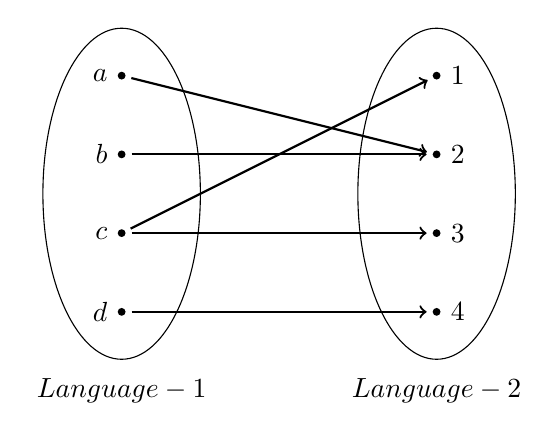
\begin{tikzpicture}[ele/.style={fill=black,circle,minimum width=.8pt,inner sep=1pt},every fit/.style={ellipse,draw,inner sep=-2pt}]

\node at (0,0) {$Language-1$};
\node at (4,0) {$Language-2$};
  \node[ele,label=left:$a$] (a1) at (0,4) {};    
  \node[ele,label=left:$b$] (a2) at (0,3) {};    
  \node[ele,label=left:$c$] (a3) at (0,2) {};
  \node[ele,label=left:$d$] (a4) at (0,1) {};

  \node[ele,,label=right:$1$] (b1) at (4,4) {};
  \node[ele,,label=right:$2$] (b2) at (4,3) {};
  \node[ele,,label=right:$3$] (b3) at (4,2) {};
  \node[ele,,label=right:$4$] (b4) at (4,1) {};

  \node[draw,fit= (a1) (a2) (a3) (a4),minimum width=2cm] {} ;
  \node[draw,fit= (b1) (b2) (b3) (b4),minimum width=2cm] {} ;  
  %\draw[->,thick,shorten <=2pt,shorten >=2pt] (a1) -- (b4);
  \draw[->,thick,shorten <=2pt,shorten >=2] (a1) -- (b2);
  \draw[->,thick,shorten <=2pt,shorten >=2] (a2) -- (b2);
  \draw[->,thick,shorten <=2pt,shorten >=2] (a3) -- (b1);
  \draw[->,thick,shorten <=2pt,shorten >=2] (a3) -- (b3);
  \draw[->,thick,shorten <=2pt,shorten >=2] (a4) -- (b4);
 \end{tikzpicture}

\caption{Visualization of translations}
\label{fig:function}
\end{figure}

\begin{conf}{Functions}
	To be honest, it's easiest to think of translations as methods, and less like functions. Most students tend to think of translatons as functions, where they're just mappings in which one input (in Language 1) maps to a unique translation in Language 2. However, this is hardly true. In the majority of cases, one input can map to several outputs, and one output can map to several inputs (as shown in figure~\ref{fig:function}). Sometimes, a translation of a particular sentence or phrase is a one-to-one mapping, but this doesn't happen as frequently as we'd hope.
\end{conf}

Use \ita{cualquier} when the meaning is somewhere between ``any'' and ``whichever.''
\subsection{Wherever}

With translating the idea of ``wherever,'' we have a few different options, where we can choose to use the subjunctive or the indicative. 

\subsubsection{With subjunctive}
With the subjunctive, ``wherever'' works just as ``whatever'' worked, with a bit of a difference. Remember how there are two different ways to ask where, \ita{d\'onde} and \ita{a d\'onde/ad\'onde}\footnote{Within this guide, I'm going to be using \ita{adonde}, not \ita{a donde}}? When we translate ``whenever,'' keep in mind whether we need to indicate movement. \\

Within this subcategories, we have a couple of different options. 
The idea of ``wherever'' can be translated as \ita{donde/adonde + verbo} or \ita{dondequiera/adondequiera que + verbo}, where the verb is conjugated in the subjunctive mood. \footnote{For the latter option, the verb in question is typically \ita{ser}.} \\

Now, our decision tree branches out a bit. In most cases, we use the \ita{donde/adonde + verbo} option. In more formal examples, such as in poetry or literature, we can use \ita{dondequiera/adondequiera que + verbo}. \\

For example, the sentence ``We can eat wherever you want'' can be translated as \ita{Podemos comer donde quieras} or \ita{Podemos comer dondequiera que sea.} The first sentence is used for most part, but the second sentence can be used in more formal contexts. Note that we're using the form related to the pronoun \ita{donde}, since we don't need to indicate movement. \\

However, if we wanted to translate the sentence ``The frogs followed the insects wherever they went,'' we could say \ita{Las ranas siguieron los insectos adonde fueran/fuesen} or \ita{Las ranas siguieron los insectos adondequiera que fueran/fuesen.} Here, since we need to indicate the frogs' movement toward the insects, we're using the \ita{adonde} form. 

\subsubsection{Without subjunctive}
There's also a small hack we can use to convey the idea of ``wherever'' without using the subjunctive: using \hyperref[subsec:cualquier]{\ita{cualquier}}. We can say \ita{cualquier lugar/sitio/parte}. 

\subsection{Whenever}

This section is pretty easy, and links up with the \hyperref[sec:relpro]{Usage with other relative pronouns} section. 

\subsection{Whoever}
Let's move on to whoever, which can be translated as \ita{quienquiera que ...}. For example, the sentence  ``Whoever you are/may be, please leave'' can be translated as \ita{Quienquiera que seas, por favor salga.} \footnote{I've chosen to use the formal command in this case, since the speaker obviously doesn't know who they're addressing.}\\

\subsubsection{Anyone}
This is also a good time to talk about the phrase ``anyone'' or ``anybody,'' 


The word \ita{cualquiera} follows \hyperref[sec:apo]{apocapation}. 

\section{Even if/though}

\ita{Aunque} can either be translated as ``even if'' or ``even though.'' \ita{Por m\'as que} can be translated as \ita{However ... it may be}. If the speaker feels pretty certain about what's about to follow, use the indicative. Else, use the subjunctive. However, you'll typically find that \ita{aunque} and \ita{por m\'as que} are \underline{typically} used with the subjunctive. \\

Let's look at a few sample sentences: 
\begin{enumerate}[noitemsep]
	\item ``Even if it's hard, don't give up.''/``However hard it may be, don't give up.'' \arr
		\begin{itemize}[noitemsep]
			\item \ita{Aunque sea dif\'icil, no te rindas.}
			\item \ita{Por m\'as dif\'icil que sea, no te rindas.}
		\end{itemize}
	\item ``Even though the clay pot broke, I enjoyed making it.'' \arr \ita{Aunque el tarro de arcilla se rompi\'o, disfrut\'e cre\'andolo.}
\end{enumerate}

\section{In case ...}

%\newpage
\chapter{Always, Sometimes, Never}
Remember how in previous sections, we talked about how some instances:
\begin{itemize}
	\item will require you to use the indicative
	\item will require you to use the subjunctive
	\item or leave it to the speaker to pick the mood?
\end{itemize}

The following table is a quick overview of which of those conditions apply, by telling you when to use the subjunctive. \\

\begin{itemize}
	\item \underline{Always} means that if you see that expression, the corresponding verb will be conjugated in the subjunctive mood
	\item \underline{Never} means that if you see that expression, the corresponding verb will be conjugated in the indicative mood
	\item \underline{Sometimes} means that other factors come into play when it comes to deciding which mood to use
\end{itemize}

\begin{table}[H]
	\centering
	\begin{tabular}{llll}
	\toprule
	 & \textbf{Always} & \textbf{Sometimes} & \textbf{Never} \\
	\midrule
	Wishes & \checkmark & & \\
	Emotional Expressions & & \checkmark & \\
	Impersonal Expressions with two clauses  & \checkmark & &\\
	Impersonal Expressions with only one clause& & &  \checkmark\\
	Recommendations & \checkmark & & \\
	Doubt \& Denial & &  \checkmark & \\
	\ita{Ojal\'a} & \checkmark & & \\
	\ita{Si}-Clauses, subordinate clause in conditional & \checkmark & & \\
	\ita{Si}-Clauses, subordinate clause in present indicative & & & \checkmark \\
	What if? & \checkmark & & \\
	Maybe & & \checkmark & \\
	So that ... & \checkmark & & \\
	\ita{Sin que} & \checkmark & & \\
	Unless & \checkmark & & \\
	Provided/given that & \checkmark & & \\
	Time expressions in the past & & & \checkmark \\
	Time expression in the present/future & \checkmark & & \\
	Other relative pronouns & & \checkmark & \\
	Expressions of certainty & & & \checkmark \\
	Directly after a preposition & & & \checkmark \\
	Even if/though & & \checkmark & \\
	However .. it may be & & \checkmark & \\
	Despite & & & \checkmark  \\
	Whoever & \checkmark & & \\
	Whatever & \checkmark & & \\
	Whichever & & & \checkmark \\
	Whenever & \checkmark & & \\
	Wherever & & \checkmark & \\

	\bottomrule
	\end{tabular}
	\caption{Always, Sometimes, and Never}
\end{table}

\chapter{Additional Practice}
Translate the following sentences.\\

Remember to think through whether the subjunctive and/or the indicative is used. If there are multiple correct translations, it can be helpful to think about all of them, and think about whether the meaning changes. \ita{\textexclamdown Buena suerte!}\\

Answers are given in the \hyperref[sec:ans]{Answers} section.

\begin{enumerate}
	\item If I had a million dollars, I'd build a frog sanctuary. 
	\item Maybe you should rest.
	\item When I'm older, I'm going to have a frog.
	\item I'm writing this guide so that you'll understand the subjunctive. 
	\item Unless you're sick, you should attend the meeting.
	\item I want to block certain users, so that they cannot see my posts.
	\item I want you to finish your chores before I get home. 
	\item You finished your chores before I got home.
	\item In case you need help, call me!
	\item We can do the project whenever we feel like it. 
	\item Even though I got a bad grade on the project, I learnt a lot.
	\item What if the car broke down?
	\item I'll do whatever/anything you want.
	\item I read the secret novels without them knowing. 
	\item Given that frogs are cute, we should not hurt them.
	\item I want to speak with someone who understands me.
\end{enumerate}

%\newpage
\chapter{Answers}
\label{sec:ans}

\section{Answers to Conjugation Practice}
\subsection{Present Subjunctive}

\conjugation[
	caption=Present subjunctive conjugation of \textit{tener},
	label=verb:tener
]{tenga \\ tengas \\ tenga \\ tengamos \\ teng\'ais \\ tengan}


\conjugation[
	caption=Present subjunctive conjugation of \textit{dar},
	label=verb:dar
]{d\'e \\ des \\ d\'e \\ demos \\ deis \\ den}

\conjugation[
	caption=Present subjunctive conjugation of \textit{saber},
	label=verb:saber
]{sepa \\ sepas \\ sepa \\ sepamos \\ sep\'ais \\ sepan}

\conjugation[
	caption=Present subjunctive conjugation of \textit{averiguar},
	label=verb:averiguar
]{averig\"ue \\ averig\"ues \\ averig\"ue \\ averig\"uemos \\ averig\"ueis \\ averig\"uen}


\conjugation[
	caption=Present subjunctive conjugation of \textit{poner},
	label=verb:poner
]{ponga \\ pongas \\ ponga \\ pongamos \\ pong\'ais \\ pongan}


\conjugation[
	caption=Present subjunctive conjugation of \textit{escribir},
	label=verb:escribir
]{escriba \\ escribas \\ escriba \\ escribamos \\ escrib\'ais \\ escriban}


\conjugation[
	caption=Present subjunctive conjugation of \textit{levantar},
	label=verb:levantar
]{levante \\ levantes \\ levante \\ levantemos \\ levant\'eis \\ levanten}


\conjugation[
	caption=Present subjunctive conjugation of \textit{bajar},
	label=verb:bajar
]{baje \\ bajes \\ baje \\ bajemos \\ baj\'eis \\ bajen}

\conjugation[
	caption=Present subjunctive conjugation of \textit{hacer},
	label=verb:hacer
]{haga \\ hagas \\ haga \\ hagamos \\ hag\'ais \\ hagan}


\conjugation[
	caption=Present subjunctive conjugation of \textit{colocar},
	label=verb:colocar
]{coloque \\ coloques \\ coloque \\ coloquemos \\ coloqu\'eis \\ coloquen}

\conjugation[
	caption=Present subjunctive conjugation of \textit{empezar},
	label=verb:empezar
]{empiece \\ empieces \\ empiece \\ empecemos \\ empec\'eis \\ empiecen}


\conjugation[
	caption=Present subjunctive conjugation of \textit{leer},
	label=verb:leer
]{lea \\ leas \\ lea \\ leamos \\ le\'ais \\ lean}

%%%%%%%%%%%%%%%%%%%%%%%%%%%%%%%%%%%%%%%%%%%%%%%%%%%%%%%%%%%%%%%%%%%%%%%%%%%%%%%
\subsection{Subjunctive Imperfect}

\conjugation[
	caption=Subjunctive imperfect conjugation of \textit{entender},
	label=verb:entender
]{entendie+ra/se \\ entendie+ras/ses \\ entendie+ra/se \\ entendi\'e+ramos/semos \\ entendie+rais/seis \\ entendie+ran/sen}

\conjugation[
	caption=Subjunctive imperfect conjugation of \textit{ser},
	label=verb:ser
]{fue+ra/se \\ fue+ras/ses \\ fue+ra/se \\ fu\'e+ramos/semos \\ fue+rais/seis \\ fue+ran/sen}

\conjugation[
	caption=Subjunctive imperfect conjugation of \textit{andar},
	label=verb:andar
]{anduvie+ra/se \\ anduvie+ras/ses \\ anduvie+ra/se \\ anduvi\'e+ramos/semos \\ anduvie+rais/seis \\ anduvie+ran/sen}

\conjugation[
	caption=Subjunctive imperfect conjugation of \textit{estar},
	label=verb:estar
]{estuvie+ra/se \\ estuvie+ras/ses \\ estuvie+ra/se \\ estuvi\'e+ramos/semos \\ estuvie+rais/seis \\ estuvie+ran/sen}

\conjugation[
	caption=Subjunctive imperfect conjugation of \textit{convertir},
	label=verb:convertir
]{convirtie+ra/se \\ convirtie+ras/ses \\ convirtie+ra/se \\ convirti\'e+ramos/semos \\ convirtie+rais/seis \\ convirtie+ran/sen}

\conjugation[
	caption=Subjunctive imperfect conjugation of \textit{decir},
	label=verb:decir
]{dije+ra/se \\ dije+ras/ses \\ dije+ra/se \\ dij\'e+ramos/semos \\ dije+rais/seis \\ dije+ran/sen}

\conjugation[
	caption=Subjunctive imperfect conjugation of \textit{venir},
	label=verb:venir
]{vinie+ra/se \\ vinie+ras/ses \\ vinie+ra/se \\ vini\'e+ramos/semos \\ vinie+rais/seis \\ vinie+ran/sen}

\conjugation[
	caption=Subjunctive imperfect conjugation of \textit{saber},
	label=verb:saber
]{supie+ra/se \\ supie+ras/ses \\ supie+ra/se \\ supi\'e+ramos/semos \\ supie+rais/seis \\ supie+ran/sen}


\conjugation[
	caption=Subjunctive imperfect conjugation of \textit{bailar},
	label=verb:bailar
]{baila+ra/se \\ baila+ras/ses \\ baila+ra/se \\ bail\'a+ramos/semos \\ baila+rais/seis \\ baila+ran/sen}

\conjugation[
	caption=Subjunctive imperfect conjugation of \textit{querer},
	label=verb:querer
]{quisie+ra/se \\ quisie+ras/ses \\ quisie+ra/se \\ quisi\'e+ramos/semos \\ quisie+rais/seis \\ quisie+ran/sen}




\section{Answers to Practice \#1}
\begin{enumerate}
	\item \ita{Me dijo que lavara/lavase los platos. }
	\item \ita{Espero ganar una medalla de oro en la competencia.}
	\item \ita{Espero que ganes una medalla de oro en la competencia.}
	\item \ita{Estoy segur@ de que todo saldr\'a bien.}
	\item \ita{Ojal\'a fuera una rana.}
	\item \ita{Es terrible que las ranas se mueran.}
	\item \ita{Prefiero que escribas con pluma, y no con l\'apiz.}
	\item \ita{Me forzaron limpiar mi cuarto.}
	\item \ita{Es malo mentir.}
	\item \ita{Cre\'ia que vendr\'ia.}
	\item \ita{Dudaba que llegara a tiempo.}

\end{enumerate}
\section{Answers to Practice \#2}

%\newpage
\chapter{Appendix}
\label{sec:appendix}
\section{List of Tenses and Moods}
\label{subsec:tense}
\textbf{Indicative Mood}
	\begin{itemize}[noitemsep]
		\item Simple Present (\textit{el presente simple})
		\item Past Perfect/Preterit (\textit{el pasado perfecto/el pret\'{e}rito })
		\item Imperfect (\textit{el imperfecto})
		\item Conditional (\textit{el condicional})
		\item Future (\textit{el futuro})
		\item Corresponding perfect tenses:
			\begin{itemize}[noitemsep]
				\item Present perfect (\textit{el presente perfecto})
				\item Preterit perfect (\textit{el pret\'{e}rito perfecto})
				\item Past perfect (\textit{el pasado perfecto})
				\item Conditional perfect (\textit{el condicional perfecto})
				\item Future perfect (\textit{el futuro perfecto})
			\end{itemize}
	\end{itemize}

\textbf{Subjunctive Mood}
	\begin{itemize}[noitemsep]
		\item Simple Present (\textit{el presente simple})
		\item Imperfect 1 \& 2 (\textit{el imperfecto 1 \& 2}) 
		\item Future (\textit{el futuro})
		\item Corresponding perfect tenses in the subjunctive:
			\begin{itemize}[noitemsep]
				\item Subjunctive present perfect (\textit{el presente perfecto del subjuntivo}) 
				\item Subjunctive past perfect 1 \& 2 (\textit{el pasado perfecto del subjuntivo 1 \& 2})
				\item Subjunctive conditional perfect (\textit{el condicional perfecto del subjuntivo})
				\item Subjunctive future perfect (\textit{el futuro perfecto del subjuntivo})
			\end{itemize}
	\end{itemize}

\textbf{Imperative Mood}
	\begin{itemize}[noitemsep]
		\item There's only really a present tense form. However, there are two sub-forms (not tenses):
			\begin{itemize}[noitemsep]
				\item Affirmative (\textit{afirmativo}): used to tell people to do something
				\item Negative (\textit{negativo}): used to tell people \underline{not} to do something
			\end{itemize}
	\end{itemize}

\section{Pronunciation and Spelling Rules}
\label{subsec:pronun}

Spanish is a pretty phonetic language, which is a blessing for students. This subsection isn't a comprehensive pronunciation or spelling guide, but it covers the reasons why we need to change the spelling of certain conjugated verbs. 

\subsection{C,G, and Z}
In this subsubsection, we're going to look into spelling changes related to \ita{-car}, \ita{-gar}, \ita{-zar}, and \ita{-guar} verbs . \\ 

In Spanish, the letter \ita{c} can be pronounced in two ways: like an English ``s'' or an English ``k.'' How do we know which pronunciation to use? It entirely depends on what letter follows the \ita{c}. 
\begin{itemize}[noitemsep]
	\item Consonant follows? Pronounce it like a ``k.''
	\item Vowel follows? It depends. Followed by an 
		\begin{itemize}[noitemsep]
			\item \ita{a, o} or \ita{u}? Pronounce it like a ``k.''
			\item \ita{e} or \ita{i}? Pronounce it like a ``s.''
		\end{itemize}
\end{itemize}

The exact same set of rules apply to the pronunciation of the letter \ita{g}. In Spanish, the letter \ita{g} can be pronounced either as a hard ``g'' sound (like in the word ``goat,'' written as /g/), or similar to the \ita{j} in Spanish (the \ita{jota}, written as /x/).\footnote{In linguistics, the former is a voiced velar fricative and the latter is a voiceless velar fricative, if you're curious.} Let's go through the same decision tree: 
\begin{itemize}[noitemsep]
	\item Consonant follows? Pronounce it like a /g/ 
	\item Vowel follows? It depends. Followed by an 
		\begin{itemize}[noitemsep]
			\item \ita{a, o} or \ita{u}? Pronounce it like a /g/
			\item \ita{e} or \ita{i}? Pronounce it like a /x/
		\end{itemize}
\end{itemize}

\begin{conf}{You'll be okay. }
To be honest, this tree can kinda seem intimidating at first. Most Spanish speakers don't use anything like this tree to talk. I highly recommend listening to native sources and repeating words and phrases to get more comfortable with pronunciation. This tree is just there to help you out in a moment of need, if you don't know how to pronounce a certain letter. I wouldn't really expect it to carry you through a conversation.
\end{conf}

Now that we've gone over that, what does it have to do with spelling changes?\\

Let's take the example verb \ita{buscar} (to look for), and we're going to conjugate it in the present subjunctive. 
First, let's look at the pronunciation of the \ita{c} in \ita{buscar}. Since the \ita{c} is followed by an \ita{a}, the \ita{c} will be pronounced like the English ``k.''i\\

Next, following the steps, we'd eventually wind up at \sout{\ita{busce}}. If you look at how the letter \ita{c} is pronounced in the fake word \sout{\ita{busce}}, you'll find that the \ita{c} would be pronounced as an English ``s.'' Uh-oh. If we conjugate it like this, the \ita{c}'s pronuncuation changes from the English ``k'' to an ``s.'' Therefore, the accepted fix is to replace the \ita{c} with a \ita{qu}, so that we get \ita{busque}, which maintains the hard \ita{c} sound. \\

The same thing takes place with \ita{-gar} verbs, where the accepted fix is to add a \ita{u} after the \ita{g} to maintain pronunciation.\\ 

The case of \ita{-zar} verbs is a bit different. In Spanish, we only use the letter \ita{z} when placing the letter \ita{c} would change the pronunciation. For example, the verb \ita{alcanzar} (to reach or to acheive) could \underline{not} be written as \sout{\ita{alcancar}}, since that would be pronounced as \ita{/alkankar/}. Hence, if we don't \underline{need} to use the \ita{z}, we use the \ita{c} instead. Therefore, the \ita{z} is replaced by the \ita{c} in \ita{-zar} verb subjunctive conjugations. The verb \ita{alcanzar} would therefore be conjugated as follows in the present subjunctive:\\



\conjugation[
	caption=Present subjunctive conjugation of \textit{alcanzar},
	label=verb:empezar
]{alcance \\ alcances \\ alcance \\ alcancemos \\ alcanc\'eis \\ alcancen}


Finally, let's talk about \ita{-guar} verbs. You don't really \ita{need} to know this, since these verbs aren't super common.\\

Remember when we added a \ita{u} after the letter \ita{g} in \ita{-gar} verbs to maintain that hard /g/ sound? Keep that in mind for the rest of this paragraph. In the string \ita{gu*}, the \ita{u} is pronounced conditionally:

\begin{itemize}[noitemsep]
	\item If the letter after \ita{gu} is \ita{a, o, u}, or a consonant the \ita{u} is pronounced. 
	\item Else, the \ita{u} is not pronounced. The only purpose it serves is to maintain the hard /g/ sound. 
\end{itemize}

In verbs like \ita{averiguar} (to find out), if we were to follow previously
defined subjunctive conjugation rules, we'd get \sout{\ita{averigue}}. In the
original verb \ita{averiguar}, the \ita{u} is indeed pronounced, while in the
conjugated version we (incorrectly) generated, the \ita{u} would not be
pronounced. Hence, the fix is to add a \ita{diaresis} to the \ita{u}, to
indicate that we should pronounce it.\footnote{This breaks up what would have
been a diphthong, creating a hiatus.} Our final result should be \ita{averig{\"u}e}.

\subsection{Accent Rules}
\label{subsec:accents}
This is probably my favorite aspect of the Spanish language. I really hope it becomes your favorite too, once you understand it.\\

\begin{conf}{Way to Approach This}
	Before we dive in, here's a quick bit of advice. This part of Spanish really exemplifies what language ``rules'' really are about. Most folks tend to think of them as super prescriptive and rigid laws that are to be followed at all costs, but that idea couldn't be more wrong. Language ``rules'' are really just a set of patterns that evolves just as the language itself evolves. In linguistics, the only thing that's truly \ita{wrong} would be something a native speaker would never say. What's wrong or right does not follow these rules; the rules follow the speakers. The beauty about Spanish pronunciation/spelling is that the spelling \ita{follows} the pronunciation - the written form evolved along with the spoken form.  
\end{conf}

Rant over; let's jump right in. In Spanish, accent marks can serve two purposes: they indicate which syllable should be stressed, or they're used to distinguish between words that would otherwise be written and said identically. \\

First, let's go over stress rules.\\

\begin{conf}{The Golden Rules}
If a word ends in either an \ita{n}, \ita{s}, or a vowel, the penultimate syllable of the word will be stressed. Else, the last syllable of the word is stressed. If the above two statements are not true for a word (meaning the stress falls elsewhere), the word will have an accent mark.
\end{conf}

Let's go through a couple of example words: \ita{alem{\'a}n} (German, m. s.) and \ita{alemana} (German, f. s.).\\

Let's first start out with \sout{\ita{aleman}}, a word that doesn't exist. In the masculine singular adjective for German, the stress falls on the vowel between the \ita{m} and the \ita{n}. However, since our fake word  \sout{\ita{aleman}} ends in an \ita{n}, the second-to-last syllable (the \ita{e}) will be stressed, which does \underline{not} match the spelling. Therefore, we'll need to add an accent mark on the last syllable, so that we get \ita{alem{\'a}n}. \\

Now let's move on to the feminine singular adjective for German, \ita{alemana}.
The stress on this word falls on the same place as it did in the word
\ita{alem{\'a}n}, the vowel between the \ita{m} and the \ita{n}. Since this word
ends in a vowel, the stress already falls on the appropriate vowel (the
\ita{a} between the \ita{m} and the \ita{n}). Hence, we don't need to add a
diacritic to indicate where the stress falls; we already know since it follows
the ``Golden Rules.''\\

Finally, let's go over a case where the addition of an accent mark is not for the purpose of changing pronunciation; rather, the accent mark just helps us distinguish between words that would otherwise be spelled identically. A subjunctive conjugation of the verb \ita{dar} (to give) is \ita{d{\'e}}. This is used to distinguish it from the preposition \ita{de} (of, from). Another example of this usage of an accent mark is in the word \ita{s{\'i}} (yes), which, without the accent mark, could be confused with \ita{si} (if).

\section{Apocapation}
\label{sec:apo}

Let's learn some fun linguistics stuff! \\

Apocapation is shortening the last bit of a word, and we do it pretty frequently
even in English. For example, we tend to say ``lab'' instead of ``laboratory,''
and ``intro'' instead of ``introduction.'' In Spanish, the use of these apocopes
is sometimes \underline{required}. In this section, we'll mainly be discussing
situations where we don't really have a choice. \\

In many cases, we just do it to \underline{certain} adjectives in the masculine singular form before nouns, but in some cases, we do it for the feminine singular form too, in the word \ita{grande} for instance.\\

\subsection {Masculine Singular Apocopes}
Let's look at the adjective \ita{primero} (first):
\begin{table}[ht]
\centering
\begin{tabular}[t]{lll}
\toprule
&Masculine&Feminine\\
\midrule
	Singular&\ita{primero}&\ita{primera}\\
	Plural& \ita{primeros}&\ita{primeras}\\
\bottomrule
\end{tabular}
	\caption{Inflections of \ita{primero}}
\end{table}

Therefore, the sentence ``The first car is the best,'' we would say \ita{El primer coche es el mejor}, instead of \sout{\ita{El primero coche es el mejor}}. \\

If you look at the table above, and the previous sentence, you might be wondering when we actually use the form \ita{primero}. We use that form when the adjective isn't actually placed before the noun. For example, in the sentence, ``He was the first to get up'' (\ita{Fue el primero en levantarse}), there's no noun after the adjective, so the long form, \ita{primero}, is used. We also use this long form in dates, such as to say ``the first of August'' (\ita{el primero de agosto}). Lastly, we use this form as an adverb, like when we say ``First, let's sit down'' (\ita{Primero, vamos a sentarnos}). \\

In the majority of cases, like for the word \ita{primero}, we only have to use the short form when we're describing masculine singular objects. The following is an exhaustive list of adjectives that only change in the \underline{masculine singular form}. \\

\begin{table}[H]
\centering
	\begin{tabular}[!htbp]{lll}
\toprule
		\textbf{Adjective }& \textbf{Apocope}& \textbf{Meaning}\\
\midrule
	\ita{uno} & \ita{un} & a/an \\
	\ita{alguno} & \ita{alg\'un} & some/any \\
	\ita{ninguno} & \ita{ning\'un} & no/none \\
	\ita{bueno}&\ita{buen}&good\\
	\ita{malo} & \ita{mal} & bad\\
	\ita{primero}& \ita{primer}& first\\
	\ita{tercero} & \ita{tercer} & third \\
	\ita{postrero} & \ita{postrer} & last \\

\bottomrule
\end{tabular}
	\caption{Exhaustive list of masculine singular apocopes}
\end{table}

\subsection{\ita{Grande}}
The adjective \ita{grande} works slightly differently from the apocopes we just saw, adjectives that only change in the masculine singular form. With \ita{grande} use the short adjective \ita{gran} in front of both masculine and feminine singular nouns. Therefore, we would say \ita{El Gran Juego} and \ita{una gran aventura}. \\

Remember, \ita{grande} means ``great'' when it's placed \underline{before} a noun. It means ``large'' when it's placed after a noun.


\subsection{\ita{Santo}}

This one's pretty easy. For male saints whose names do not begin with \ita{To-} or \ita{Do-}, use the short form \ita{San.} For male saints whose names begin with \ita{To-} or \ita{Do-}, use the long form \ita{Santo} \footnote{The reason for this is to avoid confusion. Saying \sout{\ita{San Tom\'as}} could sound like \sout{\ita{Santo mas}}.}. \\

Therefore, we'd say \ita{San Mart\'in} and \ita{San Miguel}, but we'd say \ita{Santo Tom\'as} or \ita{Santo Domingo.}

\subsection{\ita{Ciento}}
This one's also pretty easy. We use \ita{ciento} if it's followed by another number; for example, to say ``102 frogs'', we'd say \ita{ciento dos ranas}. Else, use the shortened form \ita{cien}. For example, we'd say \ita{cien ranas} (100 frogs) or \ita{cien mill\'on ranas} (100 million frogs). 

\subsection{\ita{Cualquiera}}

\ita{Cualquiera} is a pronoun that means ``anyone,'' in the sense of ``whichever human.'' For example, we could say \ita{Cualquiera puede cocinar} (Anyone can cook). \footnote{I feel oddly nostalgic and wish to watch Ratatouille for the millionth time.}  \\

\ita{Cualquier/Cualesquier}, the corresponding apocope, means ``any,'' in the sense of ``whichever one(s).'' For example, we could translate the sentence ``It doesn't really matter, you can pick whatever you want'' as \ita{Me da igual; puedes elegir cualquier cosa que quieras}. For instance, we could translate the sentence ``You can do it any way you like'' as \ita{Puedes hacerlo en cualquier forma},``You can do it in any way you like.''

\subsection{\ita{Tanto}}

Last, but not least, let's address the word \ita{tanto}, which means ``so much'' or ``so many.'' Remember that this word is typically used an adjective, so we tend to use it with reference to a given noun. Here are its inflections:  
\begin{table}[ht]
\centering
\begin{tabular}[t]{lll}
\toprule
&Masculine&Feminine\\
\midrule
	Singular&\ita{tanto}&\ita{tanta}\\
	Plural& \ita{tantos}&\ita{tantas}\\
\bottomrule
\end{tabular}
	\caption{Inflections of \ita{tanto}}
\end{table}

Hence, the following are all valid sentences:
\begin{enumerate}[noitemsep]
	\item \ita{Tengo tanto trabajo que hacer.} \arr ``I have so much work to do.''
	\item \ita{!`Hay tanta gente!} \arr ``There are so many people!''
	\item \ita{He cometido tantos errores.} \arr ``I've made so many mistakes.'
	\item \ita{Hay tantas maneras de resolver este problema.} \arr ``There are so many ways of solving this problem.''
\end{enumerate}

The word \ita{tanto} (this time unchanging) can also be used as an adverb, like in the sentence \ita{Te extra\~no tanto} (I miss you so much). \\

Let's now move on to the apocope, \ita{tan}. \ita{Tan} is the adverb, and means ``so.'' For instance, we could translate ``Frogs are so important to her'' as \ita{Las ranas son tan importantes para ella.}\\

Another use of both \ita{tanto} and \ita{tan} is in making comparisons. \\

We use the construction \ita{tan ... como} with adjectives and adverbs. For example, to translate the sentence ``Frogs are as cute as they are strong,'' we could say \ita{Las ranas son tan preciosas como fuertes.} \\

Using \ita{tanto} as an adverb, we use the construction \ita{tanto ... como} with verbs. For example, the sentence ``Frogs work as much as toads'' could be translated as \ita{Las ranas trabajan tanto como los sapos.}\footnote{I disagree, but that's beside the point. I'd argue that frogs are the more hard-working of the two.} \\

Finally, we use \ita{tanto} as an adjective (with nouns) in the construction \ita{tanto/a/os/as ... como}. For example, to translate the sentence \ita{Frogs have as many toes as toads}, we could say \ita{Las ranas tienen tantos dedos de pie como los sapos.}


\chapter{Thanks!}
Thank you for reading! Thank you to those that helped me learn how to use the subjunctive. Thank you to Smrithi Upadhyayula for editing it. \\ 

Here's a doodle as a token of appreciation: \footnote{Doodle made with Ti\textit{k}Z and much love. I decline to admit how long this took to make.}

\begin{center}
\begin{tikzpicture}
%\draw (0,0) parabola (4,2);
%\draw[step=1cm,gray,very thin] (-5,-5) grid (8,8);
\draw [gre] (0,0) arc (0:180:2cm);
\draw [gre] (0,0) -- (2,0);
\draw [gre] (6,0) arc (0:180:2cm);
\draw [gre] (-4,0) -- (-4,-2);
\draw [gre] (6,0) -- (6,-2);
\draw [gre] (-4,-2) .. controls (1,-5)  .. (6,-2);
\draw [gre] (-2,0) ellipse (0.5cm and 1cm); % eyeball
\draw [gre] (4,0) ellipse (0.5cm and 1cm); % eyeball
\fill[eye] (-2,-0.5) ellipse (0.3cm and 0.5cm); % eyes
\fill[eye] (4,-0.5) ellipse (0.3cm and 0.5cm); % eyes
\draw [gre] (0, -2.5) .. controls (1,-3)  .. (2,-2.5); % smile 
\draw [gre] (-1,-3.7) -- (-1,-5); % neck
\draw [gre] (3,-3.7) -- (3,-5); % neck

\draw [gre] (-1,-5) .. controls (-5,-3) and (-5,-4) .. (-0.5,-9); % legs
\draw [gre] (3,-5) .. controls (7,-3) and (7,-4) .. (2.5,-9); % legs

\draw [gre] (-0.5,-9) -- (-1, -9.5);
\draw [gre] (-1,-9.5) -- (-0.5, -9.6);
\draw [gre]  (-0.5, -9.6) -- (-0.5, -10);
\draw [gre] (-0.5, -10) -- (0.5, -9);

\draw [gre] (2.5, -9) -- (3,-9.5);
\draw [gre] (3,-9.5) -- (2.5, -9.6);
\draw [gre] (2.5, -9.6) -- (2.5, -10);
\draw [gre] (2.5, -10) -- (1.5, -9);

\draw [gre] (0.5, -9) -- (1.5, -9);

\draw [gre] (0,-5) .. controls (-1,-7) and (-1,-7) .. (0.5,-9); 
\draw [gre] (2,-5) .. controls (3,-7) and (3,-7) .. (1.5,-9); 

\filldraw[gre] (0,-1.5) circle (1pt) node[anchor=west] {};
\filldraw[gre] (2,-1.5) circle (1pt) node[anchor=west] {};%\draw (1,-5) arc (0:180:0.5cm);
\end{tikzpicture}
\end{center}


\end{document}
